\documentclass[1p]{elsarticle_modified}
%\bibliographystyle{elsarticle-num}

%\usepackage[colorlinks]{hyperref}
%\usepackage{abbrmath_seonhwa} %\Abb, \Ascr, \Acal ,\Abf, \Afrak
\usepackage{amsfonts}
\usepackage{amssymb}
\usepackage{amsmath}
\usepackage{amsthm}
\usepackage{scalefnt}
\usepackage{amsbsy}
\usepackage{kotex}
\usepackage{caption}
\usepackage{subfig}
\usepackage{color}
\usepackage{graphicx}
\usepackage{xcolor} %% white, black, red, green, blue, cyan, magenta, yellow
\usepackage{float}
\usepackage{setspace}
\usepackage{hyperref}

\usepackage{tikz}
\usetikzlibrary{arrows}

\usepackage{multirow}
\usepackage{array} % fixed length table
\usepackage{hhline}

%%%%%%%%%%%%%%%%%%%%%
\makeatletter
\renewcommand*\env@matrix[1][\arraystretch]{%
	\edef\arraystretch{#1}%
	\hskip -\arraycolsep
	\let\@ifnextchar\new@ifnextchar
	\array{*\c@MaxMatrixCols c}}
\makeatother %https://tex.stackexchange.com/questions/14071/how-can-i-increase-the-line-spacing-in-a-matrix
%%%%%%%%%%%%%%%

\usepackage[normalem]{ulem}

\newcommand{\msout}[1]{\ifmmode\text{\sout{\ensuremath{#1}}}\else\sout{#1}\fi}
%SOURCE: \msout is \stkout macro in https://tex.stackexchange.com/questions/20609/strikeout-in-math-mode

\newcommand{\cancel}[1]{
	\ifmmode
	{\color{red}\msout{#1}}
	\else
	{\color{red}\sout{#1}}
	\fi
}

\newcommand{\add}[1]{
	{\color{blue}\uwave{#1}}
}

\newcommand{\replace}[2]{
	\ifmmode
	{\color{red}\msout{#1}}{\color{blue}\uwave{#2}}
	\else
	{\color{red}\sout{#1}}{\color{blue}\uwave{#2}}
	\fi
}

\newcommand{\Sol}{\mathcal{S}} %segment
\newcommand{\D}{D} %diagram
\newcommand{\A}{\mathcal{A}} %arc


%%%%%%%%%%%%%%%%%%%%%%%%%%%%%5 test

\def\sl{\operatorname{\textup{SL}}(2,\Cbb)}
\def\psl{\operatorname{\textup{PSL}}(2,\Cbb)}
\def\quan{\mkern 1mu \triangleright \mkern 1mu}

\theoremstyle{definition}
\newtheorem{thm}{Theorem}[section]
\newtheorem{prop}[thm]{Proposition}
\newtheorem{lem}[thm]{Lemma}
\newtheorem{ques}[thm]{Question}
\newtheorem{cor}[thm]{Corollary}
\newtheorem{defn}[thm]{Definition}
\newtheorem{exam}[thm]{Example}
\newtheorem{rmk}[thm]{Remark}
\newtheorem{alg}[thm]{Algorithm}

\newcommand{\I}{\sqrt{-1}}
\begin{document}

%\begin{frontmatter}
%
%\title{Boundary parabolic representations of knots up to 8 crossings}
%
%%% Group authors per affiliation:
%\author{Yunhi Cho} 
%\address{Department of Mathematics, University of Seoul, Seoul, Korea}
%\ead{yhcho@uos.ac.kr}
%
%
%\author{Seonhwa Kim} %\fnref{s_kim}}
%\address{Center for Geometry and Physics, Institute for Basic Science, Pohang, 37673, Korea}
%\ead{ryeona17@ibs.re.kr}
%
%\author{Hyuk Kim}
%\address{Department of Mathematical Sciences, Seoul National University, Seoul 08826, Korea}
%\ead{hyukkim@snu.ac.kr}
%
%\author{Seokbeom Yoon}
%\address{Department of Mathematical Sciences, Seoul National University, Seoul, 08826,  Korea}
%\ead{sbyoon15@snu.ac.kr}
%
%\begin{abstract}
%We find all boundary parabolic representation of knots up to 8 crossings.
%
%\end{abstract}
%\begin{keyword}
%    \MSC[2010] 57M25 
%\end{keyword}
%
%\end{frontmatter}

%\linenumbers
%\tableofcontents
%
\newcommand\colored[1]{\textcolor{white}{\rule[-0.35ex]{0.8em}{1.4ex}}\kern-0.8em\color{red} #1}%
%\newcommand\colored[1]{\textcolor{white}{ #1}\kern-2.17ex	\textcolor{white}{ #1}\kern-1.81ex	\textcolor{white}{ #1}\kern-2.15ex\color{red}#1	}

{\Large $\underline{12n_{0567}~(K12n_{0567})}$}

\setlength{\tabcolsep}{10pt}
\renewcommand{\arraystretch}{1.6}
\vspace{1cm}\begin{tabular}{m{100pt}>{\centering\arraybackslash}m{274pt}}
\multirow{5}{120pt}{
	\centering
	\includegraphics[width=112pt]{../../../GIT/diagram.site/Diagrams/png/2656_12n_0567.png}\\
\ \ \ A knot diagram\footnotemark}&
\allowdisplaybreaks
\textbf{Linearized knot diagam} \\
\cline{2-2}
 &
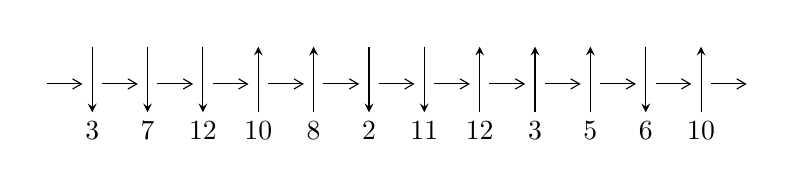
\begin{tikzpicture}[x=20pt, y=17pt]
	% nodes
	\node (C0) at (0, 0) {};
	\node (C1) at (1, 0) {};
	\node (C1U) at (1, +1) {};
	\node (C1D) at (1, -1) {3};

	\node (C2) at (2, 0) {};
	\node (C2U) at (2, +1) {};
	\node (C2D) at (2, -1) {7};

	\node (C3) at (3, 0) {};
	\node (C3U) at (3, +1) {};
	\node (C3D) at (3, -1) {12};

	\node (C4) at (4, 0) {};
	\node (C4U) at (4, +1) {};
	\node (C4D) at (4, -1) {10};

	\node (C5) at (5, 0) {};
	\node (C5U) at (5, +1) {};
	\node (C5D) at (5, -1) {8};

	\node (C6) at (6, 0) {};
	\node (C6U) at (6, +1) {};
	\node (C6D) at (6, -1) {2};

	\node (C7) at (7, 0) {};
	\node (C7U) at (7, +1) {};
	\node (C7D) at (7, -1) {11};

	\node (C8) at (8, 0) {};
	\node (C8U) at (8, +1) {};
	\node (C8D) at (8, -1) {12};

	\node (C9) at (9, 0) {};
	\node (C9U) at (9, +1) {};
	\node (C9D) at (9, -1) {3};

	\node (C10) at (10, 0) {};
	\node (C10U) at (10, +1) {};
	\node (C10D) at (10, -1) {5};

	\node (C11) at (11, 0) {};
	\node (C11U) at (11, +1) {};
	\node (C11D) at (11, -1) {6};

	\node (C12) at (12, 0) {};
	\node (C12U) at (12, +1) {};
	\node (C12D) at (12, -1) {10};
	\node (C13) at (13, 0) {};

	% arrows
	\draw[->,>={angle 60}]
	(C0) edge (C1) (C1) edge (C2) (C2) edge (C3) (C3) edge (C4) (C4) edge (C5) (C5) edge (C6) (C6) edge (C7) (C7) edge (C8) (C8) edge (C9) (C9) edge (C10) (C10) edge (C11) (C11) edge (C12) (C12) edge (C13) ;	\draw[->,>=stealth]
	(C1U) edge (C1D) (C2U) edge (C2D) (C3U) edge (C3D) (C4D) edge (C4U) (C5D) edge (C5U) (C6U) edge (C6D) (C7U) edge (C7D) (C8D) edge (C8U) (C9D) edge (C9U) (C10D) edge (C10U) (C11U) edge (C11D) (C12D) edge (C12U) ;
	\end{tikzpicture} \\
\hhline{~~} \\& 
\textbf{Solving Sequence} \\ \cline{2-2} 
 &
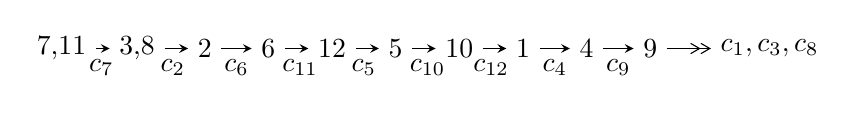
\begin{tikzpicture}[x=23pt, y=7pt]
	% node
	\node (A0) at (-1/8, 0) {7,11};
	\node (A1) at (17/16, 0) {3,8};
	\node (A2) at (17/8, 0) {2};
	\node (A3) at (25/8, 0) {6};
	\node (A4) at (33/8, 0) {12};
	\node (A5) at (41/8, 0) {5};
	\node (A6) at (49/8, 0) {10};
	\node (A7) at (57/8, 0) {1};
	\node (A8) at (65/8, 0) {4};
	\node (A9) at (73/8, 0) {9};
	\node (C1) at (1/2, -1) {$c_{7}$};
	\node (C2) at (13/8, -1) {$c_{2}$};
	\node (C3) at (21/8, -1) {$c_{6}$};
	\node (C4) at (29/8, -1) {$c_{11}$};
	\node (C5) at (37/8, -1) {$c_{5}$};
	\node (C6) at (45/8, -1) {$c_{10}$};
	\node (C7) at (53/8, -1) {$c_{12}$};
	\node (C8) at (61/8, -1) {$c_{4}$};
	\node (C9) at (69/8, -1) {$c_{9}$};
	\node (A10) at (11, 0) {$c_{1},c_{3},c_{8}$};

	% edge
	\draw[->,>=stealth]	
	(A0) edge (A1) (A1) edge (A2) (A2) edge (A3) (A3) edge (A4) (A4) edge (A5) (A5) edge (A6) (A6) edge (A7) (A7) edge (A8) (A8) edge (A9) ;
	\draw[->>,>={angle 60}]	
	(A9) edge (A10);
\end{tikzpicture} \\ 

\end{tabular} \\

\footnotetext{
The image of knot diagram is generated by the software ``\textbf{Draw programme}" developed by Andrew Bartholomew(\url{http://www.layer8.co.uk/maths/draw/index.htm\#Running-draw}), where we modified some parts for our purpose(\url{https://github.com/CATsTAILs/LinksPainter}).
}\phantom \\ \newline 
\centering \textbf{Ideals for irreducible components\footnotemark of $X_{\text{par}}$} 
 
\begin{align*}
I^u_{1}&=\langle 
5.56281\times10^{317} u^{78}-5.02067\times10^{318} u^{77}+\cdots+8.67837\times10^{319} b+1.47773\times10^{320},\\
\phantom{I^u_{1}}&\phantom{= \langle  }-3.19161\times10^{320} u^{78}+2.80481\times10^{321} u^{77}+\cdots+1.37986\times10^{322} a+2.79478\times10^{322},\\
\phantom{I^u_{1}}&\phantom{= \langle  }u^{79}-9 u^{78}+\cdots+734 u+106\rangle \\
I^u_{2}&=\langle 
2.46309\times10^{21} u^{21}-5.34185\times10^{18} u^{20}+\cdots+1.37105\times10^{22} b+2.69501\times10^{22},\\
\phantom{I^u_{2}}&\phantom{= \langle  }-1.37506\times10^{22} u^{21}+5.42032\times10^{21} u^{20}+\cdots+5.48420\times10^{22} a-2.58037\times10^{22},\\
\phantom{I^u_{2}}&\phantom{= \langle  }u^{22}+8 u^{20}+\cdots+28 u+4\rangle \\
I^u_{3}&=\langle 
b-1,\;a,\;u+1\rangle \\
I^u_{4}&=\langle 
b+1,\;a+1,\;u+1\rangle \\
\\
I^v_{1}&=\langle 
a,\;b+1,\;v+1\rangle \\
\end{align*}
\raggedright * 5 irreducible components of $\dim_{\mathbb{C}}=0$, with total 104 representations.\\
\footnotetext{All coefficients of polynomials are rational numbers. But the coefficients are sometimes approximated in decimal forms when there is not enough margin.}
\newpage
\renewcommand{\arraystretch}{1}
\centering \section*{I. $I^u_{1}= \langle 5.56\times10^{317} u^{78}-5.02\times10^{318} u^{77}+\cdots+8.68\times10^{319} b+1.48\times10^{320},\;-3.19\times10^{320} u^{78}+2.80\times10^{321} u^{77}+\cdots+1.38\times10^{322} a+2.79\times10^{322},\;u^{79}-9 u^{78}+\cdots+734 u+106 \rangle$}
\flushleft \textbf{(i) Arc colorings}\\
\begin{tabular}{m{7pt} m{180pt} m{7pt} m{180pt} }
\flushright $a_{7}=$&$\begin{pmatrix}1\\0\end{pmatrix}$ \\
\flushright $a_{11}=$&$\begin{pmatrix}0\\u\end{pmatrix}$ \\
\flushright $a_{3}=$&$\begin{pmatrix}0.0231300 u^{78}-0.203268 u^{77}+\cdots-11.9417 u-2.02541\\-0.00640998 u^{78}+0.0578527 u^{77}+\cdots-3.35031 u-1.70277\end{pmatrix}$ \\
\flushright $a_{8}=$&$\begin{pmatrix}1\\u^2\end{pmatrix}$ \\
\flushright $a_{2}=$&$\begin{pmatrix}0.0167200 u^{78}-0.145415 u^{77}+\cdots-15.2920 u-3.72818\\-0.00640998 u^{78}+0.0578527 u^{77}+\cdots-3.35031 u-1.70277\end{pmatrix}$ \\
\flushright $a_{6}=$&$\begin{pmatrix}0.0133063 u^{78}-0.111816 u^{77}+\cdots+15.5097 u+0.982850\\-0.00879467 u^{78}+0.0756675 u^{77}+\cdots-25.5253 u-6.64326\end{pmatrix}$ \\
\flushright $a_{12}=$&$\begin{pmatrix}0.0132004 u^{78}-0.125171 u^{77}+\cdots-25.7839 u-2.94270\\-0.00276583 u^{78}+0.0225513 u^{77}+\cdots-3.76731 u-0.106117\end{pmatrix}$ \\
\flushright $a_{5}=$&$\begin{pmatrix}0.0200166 u^{78}-0.171688 u^{77}+\cdots+33.7964 u+6.78443\\-0.00872034 u^{78}+0.0751173 u^{77}+\cdots-26.6187 u-6.69843\end{pmatrix}$ \\
\flushright $a_{10}=$&$\begin{pmatrix}0.00488649 u^{78}-0.0504017 u^{77}+\cdots+3.29564 u+3.47447\\-0.00255916 u^{78}+0.0228690 u^{77}+\cdots-15.8414 u-4.95528\end{pmatrix}$ \\
\flushright $a_{1}=$&$\begin{pmatrix}-0.0145289 u^{78}+0.122760 u^{77}+\cdots+14.0823 u+7.64467\\-0.0100602 u^{78}+0.0908254 u^{77}+\cdots-19.0287 u-7.67271\end{pmatrix}$ \\
\flushright $a_{4}=$&$\begin{pmatrix}0.0241505 u^{78}-0.223793 u^{77}+\cdots-42.8651 u-5.86006\\-0.00239155 u^{78}+0.0244554 u^{77}+\cdots+2.88597 u-0.413481\end{pmatrix}$ \\
\flushright $a_{9}=$&$\begin{pmatrix}0.00650299 u^{78}-0.0609618 u^{77}+\cdots+2.56028 u+1.33246\\-0.00536036 u^{78}+0.0455739 u^{77}+\cdots-8.77824 u-1.19157\end{pmatrix}$\\&\end{tabular}
\flushleft \textbf{(ii) Obstruction class $= -1$}\\~\\
\flushleft \textbf{(iii) Cusp Shapes $= -0.353846 u^{78}+3.26964 u^{77}+\cdots-551.965 u-156.813$}\\~\\
\newpage\renewcommand{\arraystretch}{1}
\flushleft \textbf{(iv) u-Polynomials at the component}\newline \\
\begin{tabular}{m{50pt}|m{274pt}}
Crossings & \hspace{64pt}u-Polynomials at each crossing \\
\hline $$\begin{aligned}c_{1}\end{aligned}$$&$\begin{aligned}
&u^{79}+43 u^{78}+\cdots+457 u+36
\end{aligned}$\\
\hline $$\begin{aligned}c_{2},c_{6}\end{aligned}$$&$\begin{aligned}
&u^{79}+u^{78}+\cdots-19 u+6
\end{aligned}$\\
\hline $$\begin{aligned}c_{3}\end{aligned}$$&$\begin{aligned}
&u^{79}-6 u^{78}+\cdots+3288 u-3153
\end{aligned}$\\
\hline $$\begin{aligned}c_{4},c_{10}\end{aligned}$$&$\begin{aligned}
&u^{79}+3 u^{78}+\cdots+39517 u+6618
\end{aligned}$\\
\hline $$\begin{aligned}c_{5}\end{aligned}$$&$\begin{aligned}
&u^{79}+12 u^{78}+\cdots+14 u+11
\end{aligned}$\\
\hline $$\begin{aligned}c_{7}\end{aligned}$$&$\begin{aligned}
&u^{79}+9 u^{78}+\cdots+734 u-106
\end{aligned}$\\
\hline $$\begin{aligned}c_{8}\end{aligned}$$&$\begin{aligned}
&u^{79}+3 u^{78}+\cdots+61 u-6
\end{aligned}$\\
\hline $$\begin{aligned}c_{9}\end{aligned}$$&$\begin{aligned}
&u^{79}+u^{78}+\cdots+18402 u+6638
\end{aligned}$\\
\hline $$\begin{aligned}c_{11}\end{aligned}$$&$\begin{aligned}
&u^{79}- u^{78}+\cdots-21 u-3
\end{aligned}$\\
\hline $$\begin{aligned}c_{12}\end{aligned}$$&$\begin{aligned}
&u^{79}-2 u^{78}+\cdots+124853 u+21439
\end{aligned}$\\
\hline
\end{tabular}\\~\\
\newpage\renewcommand{\arraystretch}{1}
\flushleft \textbf{(v) Riley Polynomials at the component}\newline \\
\begin{tabular}{m{50pt}|m{274pt}}
Crossings & \hspace{64pt}Riley Polynomials at each crossing \\
\hline $$\begin{aligned}c_{1}\end{aligned}$$&$\begin{aligned}
&y^{79}-15 y^{78}+\cdots+33889 y-1296
\end{aligned}$\\
\hline $$\begin{aligned}c_{2},c_{6}\end{aligned}$$&$\begin{aligned}
&y^{79}-43 y^{78}+\cdots+457 y-36
\end{aligned}$\\
\hline $$\begin{aligned}c_{3}\end{aligned}$$&$\begin{aligned}
&y^{79}-92 y^{78}+\cdots+324175002 y-9941409
\end{aligned}$\\
\hline $$\begin{aligned}c_{4},c_{10}\end{aligned}$$&$\begin{aligned}
&y^{79}-43 y^{78}+\cdots+1161720493 y-43797924
\end{aligned}$\\
\hline $$\begin{aligned}c_{5}\end{aligned}$$&$\begin{aligned}
&y^{79}-36 y^{78}+\cdots+2748 y-121
\end{aligned}$\\
\hline $$\begin{aligned}c_{7}\end{aligned}$$&$\begin{aligned}
&y^{79}+27 y^{78}+\cdots-45092 y-11236
\end{aligned}$\\
\hline $$\begin{aligned}c_{8}\end{aligned}$$&$\begin{aligned}
&y^{79}+27 y^{78}+\cdots+27889 y-36
\end{aligned}$\\
\hline $$\begin{aligned}c_{9}\end{aligned}$$&$\begin{aligned}
&y^{79}+91 y^{78}+\cdots-1887671940 y-44063044
\end{aligned}$\\
\hline $$\begin{aligned}c_{11}\end{aligned}$$&$\begin{aligned}
&y^{79}- y^{78}+\cdots+1149 y-9
\end{aligned}$\\
\hline $$\begin{aligned}c_{12}\end{aligned}$$&$\begin{aligned}
&y^{79}+72 y^{78}+\cdots+5381678245 y-459630721
\end{aligned}$\\
\hline
\end{tabular}\\~\\
\newpage\flushleft \textbf{(vi) Complex Volumes and Cusp Shapes}
$$\begin{array}{c|c|c}  
\text{Solutions to }I^u_{1}& \I (\text{vol} + \sqrt{-1}CS) & \text{Cusp shape}\\
 \hline 
\begin{aligned}
u &= -0.778248 + 0.684575 I \\
a &= \phantom{-}0.496147 + 0.408691 I \\
b &= -0.390677 - 0.867183 I\end{aligned}
 & -5.37716 + 3.78065 I & \phantom{-0.000000 } 0 \\ \hline\begin{aligned}
u &= -0.778248 - 0.684575 I \\
a &= \phantom{-}0.496147 - 0.408691 I \\
b &= -0.390677 + 0.867183 I\end{aligned}
 & -5.37716 - 3.78065 I & \phantom{-0.000000 } 0 \\ \hline\begin{aligned}
u &= -0.892660\phantom{ +0.000000I} \\
a &= -0.278912\phantom{ +0.000000I} \\
b &= \phantom{-}1.20837\phantom{ +0.000000I}\end{aligned}
 & \phantom{-}1.65892\phantom{ +0.000000I} & \phantom{-}7.72510\phantom{ +0.000000I} \\ \hline\begin{aligned}
u &= \phantom{-}0.135677 + 0.874172 I \\
a &= \phantom{-}2.18391 + 1.40758 I \\
b &= -1.024420 - 0.534790 I\end{aligned}
 & -2.76898 - 7.84768 I & \phantom{-}2.12757 + 8.05813 I \\ \hline\begin{aligned}
u &= \phantom{-}0.135677 - 0.874172 I \\
a &= \phantom{-}2.18391 - 1.40758 I \\
b &= -1.024420 + 0.534790 I\end{aligned}
 & -2.76898 + 7.84768 I & \phantom{-}2.12757 - 8.05813 I \\ \hline\begin{aligned}
u &= -0.781273 + 0.304744 I \\
a &= \phantom{-}0.842113 - 0.298441 I \\
b &= \phantom{-}1.265120 + 0.143006 I\end{aligned}
 & -10.97290 + 0.77841 I & -6.82766 - 0.78518 I \\ \hline\begin{aligned}
u &= -0.781273 - 0.304744 I \\
a &= \phantom{-}0.842113 + 0.298441 I \\
b &= \phantom{-}1.265120 - 0.143006 I\end{aligned}
 & -10.97290 - 0.77841 I & -6.82766 + 0.78518 I \\ \hline\begin{aligned}
u &= -0.581646 + 1.006650 I \\
a &= -0.240060 - 0.661324 I \\
b &= \phantom{-}0.185387 + 0.764265 I\end{aligned}
 & \phantom{-}4.41709 + 4.52800 I & \phantom{-0.000000 } 0 \\ \hline\begin{aligned}
u &= -0.581646 - 1.006650 I \\
a &= -0.240060 + 0.661324 I \\
b &= \phantom{-}0.185387 - 0.764265 I\end{aligned}
 & \phantom{-}4.41709 - 4.52800 I & \phantom{-0.000000 } 0 \\ \hline\begin{aligned}
u &= \phantom{-}0.804957 + 0.173139 I \\
a &= -0.302876 - 0.960865 I \\
b &= -0.935122 + 0.560283 I\end{aligned}
 & -1.36961 + 2.12804 I & -6.08728 - 3.56903 I\\
 \hline 
 \end{array}$$\newpage$$\begin{array}{c|c|c}  
\text{Solutions to }I^u_{1}& \I (\text{vol} + \sqrt{-1}CS) & \text{Cusp shape}\\
 \hline 
\begin{aligned}
u &= \phantom{-}0.804957 - 0.173139 I \\
a &= -0.302876 + 0.960865 I \\
b &= -0.935122 - 0.560283 I\end{aligned}
 & -1.36961 - 2.12804 I & -6.08728 + 3.56903 I \\ \hline\begin{aligned}
u &= -0.932036 + 0.736879 I \\
a &= -0.64902 - 1.47930 I \\
b &= -1.146240 + 0.628898 I\end{aligned}
 & -7.64208 + 9.32063 I & \phantom{-0.000000 } 0 \\ \hline\begin{aligned}
u &= -0.932036 - 0.736879 I \\
a &= -0.64902 + 1.47930 I \\
b &= -1.146240 - 0.628898 I\end{aligned}
 & -7.64208 - 9.32063 I & \phantom{-0.000000 } 0 \\ \hline\begin{aligned}
u &= -0.305349 + 0.731424 I \\
a &= -1.72358 - 0.55517 I \\
b &= \phantom{-}0.826923 + 0.741635 I\end{aligned}
 & \phantom{-}3.38241 - 1.44721 I & -0.92948 + 7.72706 I \\ \hline\begin{aligned}
u &= -0.305349 - 0.731424 I \\
a &= -1.72358 + 0.55517 I \\
b &= \phantom{-}0.826923 - 0.741635 I\end{aligned}
 & \phantom{-}3.38241 + 1.44721 I & -0.92948 - 7.72706 I \\ \hline\begin{aligned}
u &= \phantom{-}0.109380 + 0.784726 I \\
a &= \phantom{-}2.41586 - 0.71124 I \\
b &= -0.784744 + 0.443258 I\end{aligned}
 & \phantom{-}1.92515 + 0.39107 I & \phantom{-}4.91566 + 0.78548 I \\ \hline\begin{aligned}
u &= \phantom{-}0.109380 - 0.784726 I \\
a &= \phantom{-}2.41586 + 0.71124 I \\
b &= -0.784744 - 0.443258 I\end{aligned}
 & \phantom{-}1.92515 - 0.39107 I & \phantom{-}4.91566 - 0.78548 I \\ \hline\begin{aligned}
u &= -0.371146 + 0.688689 I \\
a &= \phantom{-}0.49761 + 2.75814 I \\
b &= \phantom{-}0.914340 - 0.739129 I\end{aligned}
 & \phantom{-}3.12020 + 4.18419 I & -3.46102 - 2.48442 I \\ \hline\begin{aligned}
u &= -0.371146 - 0.688689 I \\
a &= \phantom{-}0.49761 - 2.75814 I \\
b &= \phantom{-}0.914340 + 0.739129 I\end{aligned}
 & \phantom{-}3.12020 - 4.18419 I & -3.46102 + 2.48442 I \\ \hline\begin{aligned}
u &= -0.478501 + 1.123620 I \\
a &= -0.298949 + 0.824219 I \\
b &= \phantom{-}0.275465 - 0.433827 I\end{aligned}
 & \phantom{-}5.17058 + 4.04352 I & \phantom{-0.000000 } 0\\
 \hline 
 \end{array}$$\newpage$$\begin{array}{c|c|c}  
\text{Solutions to }I^u_{1}& \I (\text{vol} + \sqrt{-1}CS) & \text{Cusp shape}\\
 \hline 
\begin{aligned}
u &= -0.478501 - 1.123620 I \\
a &= -0.298949 - 0.824219 I \\
b &= \phantom{-}0.275465 + 0.433827 I\end{aligned}
 & \phantom{-}5.17058 - 4.04352 I & \phantom{-0.000000 } 0 \\ \hline\begin{aligned}
u &= \phantom{-}0.395642 + 0.656886 I \\
a &= \phantom{-}0.196734 + 0.736150 I \\
b &= -0.047600 - 0.467709 I\end{aligned}
 & \phantom{-}0.165593 - 1.209730 I & \phantom{-}2.02916 + 5.23119 I \\ \hline\begin{aligned}
u &= \phantom{-}0.395642 - 0.656886 I \\
a &= \phantom{-}0.196734 - 0.736150 I \\
b &= -0.047600 + 0.467709 I\end{aligned}
 & \phantom{-}0.165593 + 1.209730 I & \phantom{-}2.02916 - 5.23119 I \\ \hline\begin{aligned}
u &= -0.684615 + 1.041570 I \\
a &= \phantom{-}0.0285168 + 0.0826745 I \\
b &= \phantom{-}0.814198 + 0.338128 I\end{aligned}
 & \phantom{-}1.57656 - 2.62855 I & \phantom{-0.000000 } 0 \\ \hline\begin{aligned}
u &= -0.684615 - 1.041570 I \\
a &= \phantom{-}0.0285168 - 0.0826745 I \\
b &= \phantom{-}0.814198 - 0.338128 I\end{aligned}
 & \phantom{-}1.57656 + 2.62855 I & \phantom{-0.000000 } 0 \\ \hline\begin{aligned}
u &= \phantom{-}0.975838 + 0.782424 I \\
a &= \phantom{-}0.657092 - 0.713723 I \\
b &= \phantom{-}1.022580 + 0.268605 I\end{aligned}
 & -2.94747 - 3.80961 I & \phantom{-0.000000 } 0 \\ \hline\begin{aligned}
u &= \phantom{-}0.975838 - 0.782424 I \\
a &= \phantom{-}0.657092 + 0.713723 I \\
b &= \phantom{-}1.022580 - 0.268605 I\end{aligned}
 & -2.94747 + 3.80961 I & \phantom{-0.000000 } 0 \\ \hline\begin{aligned}
u &= -0.536219 + 1.134980 I \\
a &= -0.534763 - 1.106970 I \\
b &= -0.506060 + 0.508248 I\end{aligned}
 & -4.04856 + 1.41714 I & \phantom{-0.000000 } 0 \\ \hline\begin{aligned}
u &= -0.536219 - 1.134980 I \\
a &= -0.534763 + 1.106970 I \\
b &= -0.506060 - 0.508248 I\end{aligned}
 & -4.04856 - 1.41714 I & \phantom{-0.000000 } 0 \\ \hline\begin{aligned}
u &= -0.741180\phantom{ +0.000000I} \\
a &= \phantom{-}0.239372\phantom{ +0.000000I} \\
b &= \phantom{-}0.419805\phantom{ +0.000000I}\end{aligned}
 & \phantom{-}1.79441\phantom{ +0.000000I} & \phantom{-}4.83380\phantom{ +0.000000I}\\
 \hline 
 \end{array}$$\newpage$$\begin{array}{c|c|c}  
\text{Solutions to }I^u_{1}& \I (\text{vol} + \sqrt{-1}CS) & \text{Cusp shape}\\
 \hline 
\begin{aligned}
u &= \phantom{-}0.738304 + 1.048750 I \\
a &= -0.845945 - 0.269555 I \\
b &= \phantom{-}0.998142 - 0.376554 I\end{aligned}
 & -3.87655 - 1.76981 I & \phantom{-0.000000 } 0 \\ \hline\begin{aligned}
u &= \phantom{-}0.738304 - 1.048750 I \\
a &= -0.845945 + 0.269555 I \\
b &= \phantom{-}0.998142 + 0.376554 I\end{aligned}
 & -3.87655 + 1.76981 I & \phantom{-0.000000 } 0 \\ \hline\begin{aligned}
u &= \phantom{-}1.105070 + 0.664957 I \\
a &= \phantom{-}0.244803 + 0.115320 I \\
b &= -1.47554 - 0.01059 I\end{aligned}
 & -8.72804 - 7.04097 I & \phantom{-0.000000 } 0 \\ \hline\begin{aligned}
u &= \phantom{-}1.105070 - 0.664957 I \\
a &= \phantom{-}0.244803 - 0.115320 I \\
b &= -1.47554 + 0.01059 I\end{aligned}
 & -8.72804 + 7.04097 I & \phantom{-0.000000 } 0 \\ \hline\begin{aligned}
u &= \phantom{-}1.132430 + 0.621605 I \\
a &= \phantom{-}0.49514 - 1.51289 I \\
b &= -0.004512 + 0.661734 I\end{aligned}
 & -2.89071 + 3.39186 I & \phantom{-0.000000 } 0 \\ \hline\begin{aligned}
u &= \phantom{-}1.132430 - 0.621605 I \\
a &= \phantom{-}0.49514 + 1.51289 I \\
b &= -0.004512 - 0.661734 I\end{aligned}
 & -2.89071 - 3.39186 I & \phantom{-0.000000 } 0 \\ \hline\begin{aligned}
u &= -0.272017 + 0.645577 I \\
a &= -0.02750 - 1.78732 I \\
b &= -1.24922 + 0.75688 I\end{aligned}
 & -3.78506 + 8.40300 I & \phantom{-}1.55735 - 8.35283 I \\ \hline\begin{aligned}
u &= -0.272017 - 0.645577 I \\
a &= -0.02750 + 1.78732 I \\
b &= -1.24922 - 0.75688 I\end{aligned}
 & -3.78506 - 8.40300 I & \phantom{-}1.55735 + 8.35283 I \\ \hline\begin{aligned}
u &= \phantom{-}1.173230 + 0.678550 I \\
a &= \phantom{-}1.264070 + 0.058940 I \\
b &= \phantom{-}0.672858 + 0.087940 I\end{aligned}
 & -2.57246 - 4.30103 I & \phantom{-0.000000 } 0 \\ \hline\begin{aligned}
u &= \phantom{-}1.173230 - 0.678550 I \\
a &= \phantom{-}1.264070 - 0.058940 I \\
b &= \phantom{-}0.672858 - 0.087940 I\end{aligned}
 & -2.57246 + 4.30103 I & \phantom{-0.000000 } 0\\
 \hline 
 \end{array}$$\newpage$$\begin{array}{c|c|c}  
\text{Solutions to }I^u_{1}& \I (\text{vol} + \sqrt{-1}CS) & \text{Cusp shape}\\
 \hline 
\begin{aligned}
u &= \phantom{-}0.365510 + 0.529512 I \\
a &= \phantom{-}0.33616 + 1.47447 I \\
b &= -0.131837 - 1.340730 I\end{aligned}
 & -0.80564 + 1.18538 I & \phantom{-}10.43073 + 5.93489 I \\ \hline\begin{aligned}
u &= \phantom{-}0.365510 - 0.529512 I \\
a &= \phantom{-}0.33616 - 1.47447 I \\
b &= -0.131837 + 1.340730 I\end{aligned}
 & -0.80564 - 1.18538 I & \phantom{-}10.43073 - 5.93489 I \\ \hline\begin{aligned}
u &= -0.372397 + 0.523453 I \\
a &= -0.03555 + 2.76231 I \\
b &= \phantom{-}0.873019 - 0.750214 I\end{aligned}
 & \phantom{-}2.81371 + 4.24079 I & \phantom{-}1.66752 - 8.05004 I \\ \hline\begin{aligned}
u &= -0.372397 - 0.523453 I \\
a &= -0.03555 - 2.76231 I \\
b &= \phantom{-}0.873019 + 0.750214 I\end{aligned}
 & \phantom{-}2.81371 - 4.24079 I & \phantom{-}1.66752 + 8.05004 I \\ \hline\begin{aligned}
u &= \phantom{-}1.103790 + 0.828086 I \\
a &= -0.171841 - 0.938107 I \\
b &= \phantom{-}1.31594 + 0.55012 I\end{aligned}
 & -5.20033 - 4.93329 I & \phantom{-0.000000 } 0 \\ \hline\begin{aligned}
u &= \phantom{-}1.103790 - 0.828086 I \\
a &= -0.171841 + 0.938107 I \\
b &= \phantom{-}1.31594 - 0.55012 I\end{aligned}
 & -5.20033 + 4.93329 I & \phantom{-0.000000 } 0 \\ \hline\begin{aligned}
u &= -0.609086\phantom{ +0.000000I} \\
a &= -1.31379\phantom{ +0.000000I} \\
b &= -0.978193\phantom{ +0.000000I}\end{aligned}
 & -1.80797\phantom{ +0.000000I} & -4.57870\phantom{ +0.000000I} \\ \hline\begin{aligned}
u &= -0.917810 + 1.056720 I \\
a &= \phantom{-}0.327013 + 1.321270 I \\
b &= \phantom{-}1.149280 - 0.560651 I\end{aligned}
 & \phantom{-}1.73896 + 9.47414 I & \phantom{-0.000000 } 0 \\ \hline\begin{aligned}
u &= -0.917810 - 1.056720 I \\
a &= \phantom{-}0.327013 - 1.321270 I \\
b &= \phantom{-}1.149280 + 0.560651 I\end{aligned}
 & \phantom{-}1.73896 - 9.47414 I & \phantom{-0.000000 } 0 \\ \hline\begin{aligned}
u &= \phantom{-}0.313708 + 0.509032 I \\
a &= -2.16795 + 3.20848 I \\
b &= -0.923339 - 0.452097 I\end{aligned}
 & \phantom{-}1.45639 - 3.33450 I & \phantom{-}2.49781 + 7.16900 I\\
 \hline 
 \end{array}$$\newpage$$\begin{array}{c|c|c}  
\text{Solutions to }I^u_{1}& \I (\text{vol} + \sqrt{-1}CS) & \text{Cusp shape}\\
 \hline 
\begin{aligned}
u &= \phantom{-}0.313708 - 0.509032 I \\
a &= -2.16795 - 3.20848 I \\
b &= -0.923339 + 0.452097 I\end{aligned}
 & \phantom{-}1.45639 + 3.33450 I & \phantom{-}2.49781 - 7.16900 I \\ \hline\begin{aligned}
u &= -0.51363 + 1.33375 I \\
a &= \phantom{-}0.297777 + 0.674355 I \\
b &= -0.405830 - 0.317748 I\end{aligned}
 & \phantom{-}5.04693 + 3.84525 I & \phantom{-0.000000 } 0 \\ \hline\begin{aligned}
u &= -0.51363 - 1.33375 I \\
a &= \phantom{-}0.297777 - 0.674355 I \\
b &= -0.405830 + 0.317748 I\end{aligned}
 & \phantom{-}5.04693 - 3.84525 I & \phantom{-0.000000 } 0 \\ \hline\begin{aligned}
u &= \phantom{-}0.92366 + 1.16421 I \\
a &= -0.519837 + 1.155040 I \\
b &= \phantom{-}0.442033 - 1.069980 I\end{aligned}
 & -1.34186 - 10.86070 I & \phantom{-0.000000 } 0 \\ \hline\begin{aligned}
u &= \phantom{-}0.92366 - 1.16421 I \\
a &= -0.519837 - 1.155040 I \\
b &= \phantom{-}0.442033 + 1.069980 I\end{aligned}
 & -1.34186 + 10.86070 I & \phantom{-0.000000 } 0 \\ \hline\begin{aligned}
u &= \phantom{-}0.216721 + 0.462692 I \\
a &= \phantom{-}1.19356 - 4.87978 I \\
b &= -0.574841 + 0.526921 I\end{aligned}
 & -1.37094 - 3.47466 I & \phantom{-}5.22123 + 1.68240 I \\ \hline\begin{aligned}
u &= \phantom{-}0.216721 - 0.462692 I \\
a &= \phantom{-}1.19356 + 4.87978 I \\
b &= -0.574841 - 0.526921 I\end{aligned}
 & -1.37094 + 3.47466 I & \phantom{-}5.22123 - 1.68240 I \\ \hline\begin{aligned}
u &= \phantom{-}0.76744 + 1.37751 I \\
a &= \phantom{-}0.741867 - 1.057010 I \\
b &= -0.712373 + 0.831700 I\end{aligned}
 & \phantom{-}3.89746 - 2.86937 I & \phantom{-0.000000 } 0 \\ \hline\begin{aligned}
u &= \phantom{-}0.76744 - 1.37751 I \\
a &= \phantom{-}0.741867 + 1.057010 I \\
b &= -0.712373 - 0.831700 I\end{aligned}
 & \phantom{-}3.89746 + 2.86937 I & \phantom{-0.000000 } 0 \\ \hline\begin{aligned}
u &= -0.031530 + 0.417860 I \\
a &= -1.64477 - 2.92363 I \\
b &= \phantom{-}0.968462 + 0.643997 I\end{aligned}
 & \phantom{-}2.48038 - 1.25973 I & \phantom{-}0.414499 - 1.210980 I\\
 \hline 
 \end{array}$$\newpage$$\begin{array}{c|c|c}  
\text{Solutions to }I^u_{1}& \I (\text{vol} + \sqrt{-1}CS) & \text{Cusp shape}\\
 \hline 
\begin{aligned}
u &= -0.031530 - 0.417860 I \\
a &= -1.64477 + 2.92363 I \\
b &= \phantom{-}0.968462 - 0.643997 I\end{aligned}
 & \phantom{-}2.48038 + 1.25973 I & \phantom{-}0.414499 + 1.210980 I \\ \hline\begin{aligned}
u &= \phantom{-}0.10747 + 1.58916 I \\
a &= -0.00023 - 1.80456 I \\
b &= \phantom{-}0.692388 + 0.412184 I\end{aligned}
 & -4.62516 - 0.13995 I & \phantom{-0.000000 } 0 \\ \hline\begin{aligned}
u &= \phantom{-}0.10747 - 1.58916 I \\
a &= -0.00023 + 1.80456 I \\
b &= \phantom{-}0.692388 - 0.412184 I\end{aligned}
 & -4.62516 + 0.13995 I & \phantom{-0.000000 } 0 \\ \hline\begin{aligned}
u &= \phantom{-}1.04711 + 1.33119 I \\
a &= -0.04905 - 1.52114 I \\
b &= \phantom{-}1.204620 + 0.705102 I\end{aligned}
 & -3.7393 - 17.2276 I & \phantom{-0.000000 } 0 \\ \hline\begin{aligned}
u &= \phantom{-}1.04711 - 1.33119 I \\
a &= -0.04905 + 1.52114 I \\
b &= \phantom{-}1.204620 - 0.705102 I\end{aligned}
 & -3.7393 + 17.2276 I & \phantom{-0.000000 } 0 \\ \hline\begin{aligned}
u &= \phantom{-}0.90626 + 1.44153 I \\
a &= -0.03875 + 1.73006 I \\
b &= -1.004110 - 0.729834 I\end{aligned}
 & \phantom{-}2.99455 - 8.70932 I & \phantom{-0.000000 } 0 \\ \hline\begin{aligned}
u &= \phantom{-}0.90626 - 1.44153 I \\
a &= -0.03875 - 1.73006 I \\
b &= -1.004110 + 0.729834 I\end{aligned}
 & \phantom{-}2.99455 + 8.70932 I & \phantom{-0.000000 } 0 \\ \hline\begin{aligned}
u &= -0.84193 + 1.52097 I \\
a &= \phantom{-}0.286857 + 0.492815 I \\
b &= -1.040030 - 0.466600 I\end{aligned}
 & -5.72787 - 2.55886 I & \phantom{-0.000000 } 0 \\ \hline\begin{aligned}
u &= -0.84193 - 1.52097 I \\
a &= \phantom{-}0.286857 - 0.492815 I \\
b &= -1.040030 + 0.466600 I\end{aligned}
 & -5.72787 + 2.55886 I & \phantom{-0.000000 } 0 \\ \hline\begin{aligned}
u &= -1.00763 + 1.43025 I \\
a &= -0.079092 - 1.239070 I \\
b &= -1.089190 + 0.500708 I\end{aligned}
 & \phantom{-}2.88288 + 7.82891 I & \phantom{-0.000000 } 0\\
 \hline 
 \end{array}$$\newpage$$\begin{array}{c|c|c}  
\text{Solutions to }I^u_{1}& \I (\text{vol} + \sqrt{-1}CS) & \text{Cusp shape}\\
 \hline 
\begin{aligned}
u &= -1.00763 - 1.43025 I \\
a &= -0.079092 + 1.239070 I \\
b &= -1.089190 - 0.500708 I\end{aligned}
 & \phantom{-}2.88288 - 7.82891 I & \phantom{-0.000000 } 0 \\ \hline\begin{aligned}
u &= -0.231825 + 0.082340 I \\
a &= \phantom{-}1.050750 + 0.434329 I \\
b &= -1.97997 - 0.26154 I\end{aligned}
 & -0.489628 + 0.006055 I & -71.0734 - 96.8093 I \\ \hline\begin{aligned}
u &= -0.231825 - 0.082340 I \\
a &= \phantom{-}1.050750 - 0.434329 I \\
b &= -1.97997 + 0.26154 I\end{aligned}
 & -0.489628 - 0.006055 I & -71.0734 + 96.8093 I \\ \hline\begin{aligned}
u &= -0.21428 + 1.94197 I \\
a &= -0.541939 + 1.278230 I \\
b &= \phantom{-}1.006310 - 0.473935 I\end{aligned}
 & -5.75770 + 3.61725 I & \phantom{-0.000000 } 0 \\ \hline\begin{aligned}
u &= -0.21428 - 1.94197 I \\
a &= -0.541939 - 1.278230 I \\
b &= \phantom{-}1.006310 + 0.473935 I\end{aligned}
 & -5.75770 - 3.61725 I & \phantom{-0.000000 } 0 \\ \hline\begin{aligned}
u &= \phantom{-}0.99904 + 1.69268 I \\
a &= \phantom{-}0.488431 + 1.102260 I \\
b &= -1.172360 - 0.431362 I\end{aligned}
 & -6.19272 - 0.68993 I & \phantom{-0.000000 } 0 \\ \hline\begin{aligned}
u &= \phantom{-}0.99904 - 1.69268 I \\
a &= \phantom{-}0.488431 - 1.102260 I \\
b &= -1.172360 + 0.431362 I\end{aligned}
 & -6.19272 + 0.68993 I & \phantom{-0.000000 } 0 \\ \hline\begin{aligned}
u &= \phantom{-}2.15231 + 0.64578 I \\
a &= -0.203624 + 0.626602 I \\
b &= \phantom{-}1.145960 - 0.468340 I\end{aligned}
 & -5.94362 + 7.51805 I & \phantom{-0.000000 } 0 \\ \hline\begin{aligned}
u &= \phantom{-}2.15231 - 0.64578 I \\
a &= -0.203624 - 0.626602 I \\
b &= \phantom{-}1.145960 + 0.468340 I\end{aligned}
 & -5.94362 - 7.51805 I & \phantom{-0.000000 } 0\\
 \hline 
 \end{array}$$\newpage\newpage\renewcommand{\arraystretch}{1}
\centering \section*{II. $I^u_{2}= \langle 2.46\times10^{21} u^{21}-5.34\times10^{18} u^{20}+\cdots+1.37\times10^{22} b+2.70\times10^{22},\;-1.38\times10^{22} u^{21}+5.42\times10^{21} u^{20}+\cdots+5.48\times10^{22} a-2.58\times10^{22},\;u^{22}+8 u^{20}+\cdots+28 u+4 \rangle$}
\flushleft \textbf{(i) Arc colorings}\\
\begin{tabular}{m{7pt} m{180pt} m{7pt} m{180pt} }
\flushright $a_{7}=$&$\begin{pmatrix}1\\0\end{pmatrix}$ \\
\flushright $a_{11}=$&$\begin{pmatrix}0\\u\end{pmatrix}$ \\
\flushright $a_{3}=$&$\begin{pmatrix}0.250731 u^{21}-0.0988352 u^{20}+\cdots-10.6914 u+0.470510\\-0.179650 u^{21}+0.000389617 u^{20}+\cdots+0.895903 u-1.96565\end{pmatrix}$ \\
\flushright $a_{8}=$&$\begin{pmatrix}1\\u^2\end{pmatrix}$ \\
\flushright $a_{2}=$&$\begin{pmatrix}0.0710809 u^{21}-0.0984456 u^{20}+\cdots-9.79546 u-1.49514\\-0.179650 u^{21}+0.000389617 u^{20}+\cdots+0.895903 u-1.96565\end{pmatrix}$ \\
\flushright $a_{6}=$&$\begin{pmatrix}-0.0514362 u^{21}+0.155001 u^{20}+\cdots+9.60842 u+1.81921\\-0.0530987 u^{21}+0.0390748 u^{20}+\cdots-0.598343 u-5.10910\end{pmatrix}$ \\
\flushright $a_{12}=$&$\begin{pmatrix}0.124929 u^{21}+0.0291947 u^{20}+\cdots-0.0790308 u-0.197796\\0.00280485 u^{21}-0.00661764 u^{20}+\cdots-1.41274 u-0.702528\end{pmatrix}$ \\
\flushright $a_{5}=$&$\begin{pmatrix}0.101122 u^{21}+0.0831122 u^{20}+\cdots+6.07247 u+6.30830\\-0.0551212 u^{21}+0.0603063 u^{20}+\cdots+0.804315 u-4.82155\end{pmatrix}$ \\
\flushright $a_{10}=$&$\begin{pmatrix}0.225471 u^{21}+0.0177999 u^{20}+\cdots+0.799370 u+4.38328\\-0.115972 u^{21}+0.0000800783 u^{20}+\cdots-0.183112 u-4.06652\end{pmatrix}$ \\
\flushright $a_{1}=$&$\begin{pmatrix}-0.279252 u^{21}+0.0537237 u^{20}+\cdots-0.797291 u-10.8142\\0.303972 u^{21}-0.0535289 u^{20}+\cdots-3.29404 u+8.75698\end{pmatrix}$ \\
\flushright $a_{4}=$&$\begin{pmatrix}-0.345499 u^{21}-0.199154 u^{20}+\cdots-2.78153 u+1.97169\\0.0273764 u^{21}+0.148942 u^{20}+\cdots+6.18843 u-0.931880\end{pmatrix}$ \\
\flushright $a_{9}=$&$\begin{pmatrix}0.125808 u^{21}+0.0250511 u^{20}+\cdots-0.0493171 u+0.818347\\0.00109520 u^{21}-0.0353749 u^{20}+\cdots-1.45948 u-0.476329\end{pmatrix}$\\&\end{tabular}
\flushleft \textbf{(ii) Obstruction class $= 1$}\\~\\
\flushleft \textbf{(iii) Cusp Shapes $= \frac{127267665923885090334680}{13710494354785690079293} u^{21}-\frac{20268422342251723240628}{13710494354785690079293} u^{20}+\cdots-\frac{850893225143436557560740}{13710494354785690079293} u+\frac{3955364890476921757575848}{13710494354785690079293}$}\\~\\
\newpage\renewcommand{\arraystretch}{1}
\flushleft \textbf{(iv) u-Polynomials at the component}\newline \\
\begin{tabular}{m{50pt}|m{274pt}}
Crossings & \hspace{64pt}u-Polynomials at each crossing \\
\hline $$\begin{aligned}c_{1}\end{aligned}$$&$\begin{aligned}
&u^{22}-17 u^{21}+\cdots-13 u+1
\end{aligned}$\\
\hline $$\begin{aligned}c_{2}\end{aligned}$$&$\begin{aligned}
&u^{22}- u^{21}+\cdots+u-1
\end{aligned}$\\
\hline $$\begin{aligned}c_{3}\end{aligned}$$&$\begin{aligned}
&u^{22}+5 u^{21}+\cdots-6 u+1
\end{aligned}$\\
\hline $$\begin{aligned}c_{4}\end{aligned}$$&$\begin{aligned}
&u^{22}- u^{21}+\cdots-18 u+13
\end{aligned}$\\
\hline $$\begin{aligned}c_{5}\end{aligned}$$&$\begin{aligned}
&u^{22}-5 u^{21}+\cdots+2 u+1
\end{aligned}$\\
\hline $$\begin{aligned}c_{6}\end{aligned}$$&$\begin{aligned}
&u^{22}+u^{21}+\cdots- u-1
\end{aligned}$\\
\hline $$\begin{aligned}c_{7}\end{aligned}$$&$\begin{aligned}
&u^{22}+8 u^{20}+\cdots+28 u+4
\end{aligned}$\\
\hline $$\begin{aligned}c_{8}\end{aligned}$$&$\begin{aligned}
&u^{22}-5 u^{21}+\cdots+43 u-13
\end{aligned}$\\
\hline $$\begin{aligned}c_{9}\end{aligned}$$&$\begin{aligned}
&u^{22}+2 u^{21}+\cdots-12 u-4
\end{aligned}$\\
\hline $$\begin{aligned}c_{10}\end{aligned}$$&$\begin{aligned}
&u^{22}+u^{21}+\cdots+18 u+13
\end{aligned}$\\
\hline $$\begin{aligned}c_{11}\end{aligned}$$&$\begin{aligned}
&u^{22}+u^{20}+\cdots+11 u-1
\end{aligned}$\\
\hline $$\begin{aligned}c_{12}\end{aligned}$$&$\begin{aligned}
&u^{22}-5 u^{21}+\cdots-5 u-1
\end{aligned}$\\
\hline
\end{tabular}\\~\\
\newpage\renewcommand{\arraystretch}{1}
\flushleft \textbf{(v) Riley Polynomials at the component}\newline \\
\begin{tabular}{m{50pt}|m{274pt}}
Crossings & \hspace{64pt}Riley Polynomials at each crossing \\
\hline $$\begin{aligned}c_{1}\end{aligned}$$&$\begin{aligned}
&y^{22}-25 y^{21}+\cdots+11 y+1
\end{aligned}$\\
\hline $$\begin{aligned}c_{2},c_{6}\end{aligned}$$&$\begin{aligned}
&y^{22}-17 y^{21}+\cdots-13 y+1
\end{aligned}$\\
\hline $$\begin{aligned}c_{3}\end{aligned}$$&$\begin{aligned}
&y^{22}-17 y^{21}+\cdots-104 y+1
\end{aligned}$\\
\hline $$\begin{aligned}c_{4},c_{10}\end{aligned}$$&$\begin{aligned}
&y^{22}-17 y^{21}+\cdots-1546 y+169
\end{aligned}$\\
\hline $$\begin{aligned}c_{5}\end{aligned}$$&$\begin{aligned}
&y^{22}-33 y^{21}+\cdots-14 y+1
\end{aligned}$\\
\hline $$\begin{aligned}c_{7}\end{aligned}$$&$\begin{aligned}
&y^{22}+16 y^{21}+\cdots-736 y+16
\end{aligned}$\\
\hline $$\begin{aligned}c_{8}\end{aligned}$$&$\begin{aligned}
&y^{22}+17 y^{21}+\cdots-7543 y+169
\end{aligned}$\\
\hline $$\begin{aligned}c_{9}\end{aligned}$$&$\begin{aligned}
&y^{22}+8 y^{21}+\cdots-224 y+16
\end{aligned}$\\
\hline $$\begin{aligned}c_{11}\end{aligned}$$&$\begin{aligned}
&y^{22}+2 y^{21}+\cdots-163 y+1
\end{aligned}$\\
\hline $$\begin{aligned}c_{12}\end{aligned}$$&$\begin{aligned}
&y^{22}+3 y^{21}+\cdots-15 y+1
\end{aligned}$\\
\hline
\end{tabular}\\~\\
\newpage\flushleft \textbf{(vi) Complex Volumes and Cusp Shapes}
$$\begin{array}{c|c|c}  
\text{Solutions to }I^u_{2}& \I (\text{vol} + \sqrt{-1}CS) & \text{Cusp shape}\\
 \hline 
\begin{aligned}
u &= \phantom{-}0.868438 + 0.594278 I \\
a &= -1.37249 + 0.76619 I \\
b &= -0.508292 + 0.207982 I\end{aligned}
 & -2.36147 - 3.64249 I & -0.927282 + 0.923820 I \\ \hline\begin{aligned}
u &= \phantom{-}0.868438 - 0.594278 I \\
a &= -1.37249 - 0.76619 I \\
b &= -0.508292 - 0.207982 I\end{aligned}
 & -2.36147 + 3.64249 I & -0.927282 - 0.923820 I \\ \hline\begin{aligned}
u &= -0.450765 + 0.719635 I \\
a &= -0.004566 - 0.975016 I \\
b &= -0.802503 - 0.300039 I\end{aligned}
 & \phantom{-}1.20238 - 2.12854 I & -1.92738 - 0.50157 I \\ \hline\begin{aligned}
u &= -0.450765 - 0.719635 I \\
a &= -0.004566 + 0.975016 I \\
b &= -0.802503 + 0.300039 I\end{aligned}
 & \phantom{-}1.20238 + 2.12854 I & -1.92738 + 0.50157 I \\ \hline\begin{aligned}
u &= -0.339304 + 1.103900 I \\
a &= -0.472119 + 0.708930 I \\
b &= \phantom{-}0.487202 - 0.541584 I\end{aligned}
 & \phantom{-}5.32946 + 4.52303 I & \phantom{-}7.8508 - 12.4062 I \\ \hline\begin{aligned}
u &= -0.339304 - 1.103900 I \\
a &= -0.472119 - 0.708930 I \\
b &= \phantom{-}0.487202 + 0.541584 I\end{aligned}
 & \phantom{-}5.32946 - 4.52303 I & \phantom{-}7.8508 + 12.4062 I \\ \hline\begin{aligned}
u &= \phantom{-}0.207309 + 0.757040 I \\
a &= -2.32124 + 0.86023 I \\
b &= \phantom{-}0.857226 - 0.701147 I\end{aligned}
 & \phantom{-}3.69847 + 1.13168 I & \phantom{-}12.69939 + 4.46196 I \\ \hline\begin{aligned}
u &= \phantom{-}0.207309 - 0.757040 I \\
a &= -2.32124 - 0.86023 I \\
b &= \phantom{-}0.857226 + 0.701147 I\end{aligned}
 & \phantom{-}3.69847 - 1.13168 I & \phantom{-}12.69939 - 4.46196 I \\ \hline\begin{aligned}
u &= \phantom{-}0.275777 + 0.631762 I \\
a &= \phantom{-}0.71336 - 3.50085 I \\
b &= \phantom{-}0.895803 + 0.700990 I\end{aligned}
 & \phantom{-}3.57593 - 4.25665 I & \phantom{-}14.6360 + 6.2434 I \\ \hline\begin{aligned}
u &= \phantom{-}0.275777 - 0.631762 I \\
a &= \phantom{-}0.71336 + 3.50085 I \\
b &= \phantom{-}0.895803 - 0.700990 I\end{aligned}
 & \phantom{-}3.57593 + 4.25665 I & \phantom{-}14.6360 - 6.2434 I\\
 \hline 
 \end{array}$$\newpage$$\begin{array}{c|c|c}  
\text{Solutions to }I^u_{2}& \I (\text{vol} + \sqrt{-1}CS) & \text{Cusp shape}\\
 \hline 
\begin{aligned}
u &= -0.682459\phantom{ +0.000000I} \\
a &= -0.629458\phantom{ +0.000000I} \\
b &= \phantom{-}1.60199\phantom{ +0.000000I}\end{aligned}
 & \phantom{-}1.37157\phantom{ +0.000000I} & -24.7530\phantom{ +0.000000I} \\ \hline\begin{aligned}
u &= \phantom{-}1.44377 + 0.06593 I \\
a &= \phantom{-}0.196282 - 0.456604 I \\
b &= -1.193570 + 0.485737 I\end{aligned}
 & -5.37558 + 6.98207 I & \phantom{-}0.36022 - 4.86270 I \\ \hline\begin{aligned}
u &= \phantom{-}1.44377 - 0.06593 I \\
a &= \phantom{-}0.196282 + 0.456604 I \\
b &= -1.193570 - 0.485737 I\end{aligned}
 & -5.37558 - 6.98207 I & \phantom{-}0.36022 + 4.86270 I \\ \hline\begin{aligned}
u &= -0.65206 + 1.38390 I \\
a &= \phantom{-}0.646197 + 0.837522 I \\
b &= -0.633171 - 0.632803 I\end{aligned}
 & \phantom{-}5.77602 + 3.37066 I & \phantom{-}6.81116 + 0.28145 I \\ \hline\begin{aligned}
u &= -0.65206 - 1.38390 I \\
a &= \phantom{-}0.646197 - 0.837522 I \\
b &= -0.633171 + 0.632803 I\end{aligned}
 & \phantom{-}5.77602 - 3.37066 I & \phantom{-}6.81116 - 0.28145 I \\ \hline\begin{aligned}
u &= -0.38474 + 1.54379 I \\
a &= \phantom{-}0.43414 + 1.55487 I \\
b &= \phantom{-}0.685386 - 0.269781 I\end{aligned}
 & -5.07638 + 1.44838 I & -7.70492 - 3.87687 I \\ \hline\begin{aligned}
u &= -0.38474 - 1.54379 I \\
a &= \phantom{-}0.43414 - 1.55487 I \\
b &= \phantom{-}0.685386 + 0.269781 I\end{aligned}
 & -5.07638 - 1.44838 I & -7.70492 + 3.87687 I \\ \hline\begin{aligned}
u &= -0.92599 + 1.40618 I \\
a &= -0.09974 - 1.54439 I \\
b &= -1.044280 + 0.642940 I\end{aligned}
 & \phantom{-}4.47722 + 8.44438 I & \phantom{-}4.75673 - 6.97687 I \\ \hline\begin{aligned}
u &= -0.92599 - 1.40618 I \\
a &= -0.09974 + 1.54439 I \\
b &= -1.044280 - 0.642940 I\end{aligned}
 & \phantom{-}4.47722 - 8.44438 I & \phantom{-}4.75673 + 6.97687 I \\ \hline\begin{aligned}
u &= -0.138208\phantom{ +0.000000I} \\
a &= \phantom{-}2.10215\phantom{ +0.000000I} \\
b &= -2.28799\phantom{ +0.000000I}\end{aligned}
 & -0.467985\phantom{ +0.000000I} & \phantom{-}313.180\phantom{ +0.000000I}\\
 \hline 
 \end{array}$$\newpage$$\begin{array}{c|c|c}  
\text{Solutions to }I^u_{2}& \I (\text{vol} + \sqrt{-1}CS) & \text{Cusp shape}\\
 \hline 
\begin{aligned}
u &= \phantom{-}0.36790 + 1.93453 I \\
a &= -0.456168 - 1.012410 I \\
b &= \phantom{-}1.099200 + 0.373608 I\end{aligned}
 & -6.76305 - 1.34428 I & -7.76685 + 2.36036 I \\ \hline\begin{aligned}
u &= \phantom{-}0.36790 - 1.93453 I \\
a &= -0.456168 + 1.012410 I \\
b &= \phantom{-}1.099200 - 0.373608 I\end{aligned}
 & -6.76305 + 1.34428 I & -7.76685 - 2.36036 I\\
 \hline 
 \end{array}$$\newpage\newpage\renewcommand{\arraystretch}{1}
\centering \section*{III. $I^u_{3}= \langle b-1,\;a,\;u+1 \rangle$}
\flushleft \textbf{(i) Arc colorings}\\
\begin{tabular}{m{7pt} m{180pt} m{7pt} m{180pt} }
\flushright $a_{7}=$&$\begin{pmatrix}1\\0\end{pmatrix}$ \\
\flushright $a_{11}=$&$\begin{pmatrix}0\\-1\end{pmatrix}$ \\
\flushright $a_{3}=$&$\begin{pmatrix}0\\1\end{pmatrix}$ \\
\flushright $a_{8}=$&$\begin{pmatrix}1\\1\end{pmatrix}$ \\
\flushright $a_{2}=$&$\begin{pmatrix}1\\1\end{pmatrix}$ \\
\flushright $a_{6}=$&$\begin{pmatrix}0\\-1\end{pmatrix}$ \\
\flushright $a_{12}=$&$\begin{pmatrix}0\\-1\end{pmatrix}$ \\
\flushright $a_{5}=$&$\begin{pmatrix}1\\0\end{pmatrix}$ \\
\flushright $a_{10}=$&$\begin{pmatrix}1\\-1\end{pmatrix}$ \\
\flushright $a_{1}=$&$\begin{pmatrix}-1\\0\end{pmatrix}$ \\
\flushright $a_{4}=$&$\begin{pmatrix}0\\1\end{pmatrix}$ \\
\flushright $a_{9}=$&$\begin{pmatrix}1\\0\end{pmatrix}$\\&\end{tabular}
\flushleft \textbf{(ii) Obstruction class $= -1$}\\~\\
\flushleft \textbf{(iii) Cusp Shapes $= 6$}\\~\\
\newpage\renewcommand{\arraystretch}{1}
\flushleft \textbf{(iv) u-Polynomials at the component}\newline \\
\begin{tabular}{m{50pt}|m{274pt}}
Crossings & \hspace{64pt}u-Polynomials at each crossing \\
\hline $$\begin{aligned}c_{1},c_{5}\end{aligned}$$&$\begin{aligned}
&u+1
\end{aligned}$\\
\hline $$\begin{aligned}c_{2},c_{4},c_{6}\\c_{7},c_{8},c_{9}\\c_{10},c_{12}\end{aligned}$$&$\begin{aligned}
&u-1
\end{aligned}$\\
\hline $$\begin{aligned}c_{3},c_{11}\end{aligned}$$&$\begin{aligned}
&u
\end{aligned}$\\
\hline
\end{tabular}\\~\\
\newpage\renewcommand{\arraystretch}{1}
\flushleft \textbf{(v) Riley Polynomials at the component}\newline \\
\begin{tabular}{m{50pt}|m{274pt}}
Crossings & \hspace{64pt}Riley Polynomials at each crossing \\
\hline $$\begin{aligned}c_{1},c_{2},c_{4}\\c_{5},c_{6},c_{7}\\c_{8},c_{9},c_{10}\\c_{12}\end{aligned}$$&$\begin{aligned}
&y-1
\end{aligned}$\\
\hline $$\begin{aligned}c_{3},c_{11}\end{aligned}$$&$\begin{aligned}
&y
\end{aligned}$\\
\hline
\end{tabular}\\~\\
\newpage\flushleft \textbf{(vi) Complex Volumes and Cusp Shapes}
$$\begin{array}{c|c|c}  
\text{Solutions to }I^u_{3}& \I (\text{vol} + \sqrt{-1}CS) & \text{Cusp shape}\\
 \hline 
\begin{aligned}
u &= -1.00000\phantom{ +0.000000I} \\
a &= \phantom{-0.000000 } 0 \\
b &= \phantom{-}1.00000\phantom{ +0.000000I}\end{aligned}
 & \phantom{-}1.64493\phantom{ +0.000000I} & \phantom{-}6.00000\phantom{ +0.000000I}\\
 \hline 
 \end{array}$$\newpage\newpage\renewcommand{\arraystretch}{1}
\centering \section*{IV. $I^u_{4}= \langle b+1,\;a+1,\;u+1 \rangle$}
\flushleft \textbf{(i) Arc colorings}\\
\begin{tabular}{m{7pt} m{180pt} m{7pt} m{180pt} }
\flushright $a_{7}=$&$\begin{pmatrix}1\\0\end{pmatrix}$ \\
\flushright $a_{11}=$&$\begin{pmatrix}0\\-1\end{pmatrix}$ \\
\flushright $a_{3}=$&$\begin{pmatrix}-1\\-1\end{pmatrix}$ \\
\flushright $a_{8}=$&$\begin{pmatrix}1\\1\end{pmatrix}$ \\
\flushright $a_{2}=$&$\begin{pmatrix}-2\\-1\end{pmatrix}$ \\
\flushright $a_{6}=$&$\begin{pmatrix}-1\\-1\end{pmatrix}$ \\
\flushright $a_{12}=$&$\begin{pmatrix}1\\0\end{pmatrix}$ \\
\flushright $a_{5}=$&$\begin{pmatrix}-1\\-1\end{pmatrix}$ \\
\flushright $a_{10}=$&$\begin{pmatrix}1\\0\end{pmatrix}$ \\
\flushright $a_{1}=$&$\begin{pmatrix}1\\0\end{pmatrix}$ \\
\flushright $a_{4}=$&$\begin{pmatrix}0\\-1\end{pmatrix}$ \\
\flushright $a_{9}=$&$\begin{pmatrix}2\\1\end{pmatrix}$\\&\end{tabular}
\flushleft \textbf{(ii) Obstruction class $= -1$}\\~\\
\flushleft \textbf{(iii) Cusp Shapes $= -6$}\\~\\
\newpage\renewcommand{\arraystretch}{1}
\flushleft \textbf{(iv) u-Polynomials at the component}\newline \\
\begin{tabular}{m{50pt}|m{274pt}}
Crossings & \hspace{64pt}u-Polynomials at each crossing \\
\hline $$\begin{aligned}c_{1},c_{2},c_{3}\\c_{4},c_{6},c_{9}\\c_{10},c_{11}\end{aligned}$$&$\begin{aligned}
&u+1
\end{aligned}$\\
\hline $$\begin{aligned}c_{5},c_{12}\end{aligned}$$&$\begin{aligned}
&u
\end{aligned}$\\
\hline $$\begin{aligned}c_{7},c_{8}\end{aligned}$$&$\begin{aligned}
&u-1
\end{aligned}$\\
\hline
\end{tabular}\\~\\
\newpage\renewcommand{\arraystretch}{1}
\flushleft \textbf{(v) Riley Polynomials at the component}\newline \\
\begin{tabular}{m{50pt}|m{274pt}}
Crossings & \hspace{64pt}Riley Polynomials at each crossing \\
\hline $$\begin{aligned}c_{1},c_{2},c_{3}\\c_{4},c_{6},c_{7}\\c_{8},c_{9},c_{10}\\c_{11}\end{aligned}$$&$\begin{aligned}
&y-1
\end{aligned}$\\
\hline $$\begin{aligned}c_{5},c_{12}\end{aligned}$$&$\begin{aligned}
&y
\end{aligned}$\\
\hline
\end{tabular}\\~\\
\newpage\flushleft \textbf{(vi) Complex Volumes and Cusp Shapes}
$$\begin{array}{c|c|c}  
\text{Solutions to }I^u_{4}& \I (\text{vol} + \sqrt{-1}CS) & \text{Cusp shape}\\
 \hline 
\begin{aligned}
u &= -1.00000\phantom{ +0.000000I} \\
a &= -1.00000\phantom{ +0.000000I} \\
b &= -1.00000\phantom{ +0.000000I}\end{aligned}
 & -1.64493\phantom{ +0.000000I} & -6.00000\phantom{ +0.000000I}\\
 \hline 
 \end{array}$$\newpage\newpage\renewcommand{\arraystretch}{1}
\centering \section*{V. $I^v_{1}= \langle a,\;b+1,\;v+1 \rangle$}
\flushleft \textbf{(i) Arc colorings}\\
\begin{tabular}{m{7pt} m{180pt} m{7pt} m{180pt} }
\flushright $a_{7}=$&$\begin{pmatrix}1\\0\end{pmatrix}$ \\
\flushright $a_{11}=$&$\begin{pmatrix}-1\\0\end{pmatrix}$ \\
\flushright $a_{3}=$&$\begin{pmatrix}0\\-1\end{pmatrix}$ \\
\flushright $a_{8}=$&$\begin{pmatrix}1\\0\end{pmatrix}$ \\
\flushright $a_{2}=$&$\begin{pmatrix}-1\\-1\end{pmatrix}$ \\
\flushright $a_{6}=$&$\begin{pmatrix}0\\-1\end{pmatrix}$ \\
\flushright $a_{12}=$&$\begin{pmatrix}-1\\-1\end{pmatrix}$ \\
\flushright $a_{5}=$&$\begin{pmatrix}1\\-1\end{pmatrix}$ \\
\flushright $a_{10}=$&$\begin{pmatrix}0\\-1\end{pmatrix}$ \\
\flushright $a_{1}=$&$\begin{pmatrix}-1\\0\end{pmatrix}$ \\
\flushright $a_{4}=$&$\begin{pmatrix}1\\0\end{pmatrix}$ \\
\flushright $a_{9}=$&$\begin{pmatrix}0\\-1\end{pmatrix}$\\&\end{tabular}
\flushleft \textbf{(ii) Obstruction class $= 1$}\\~\\
\flushleft \textbf{(iii) Cusp Shapes $= 0$}\\~\\
\newpage\renewcommand{\arraystretch}{1}
\flushleft \textbf{(iv) u-Polynomials at the component}\newline \\
\begin{tabular}{m{50pt}|m{274pt}}
Crossings & \hspace{64pt}u-Polynomials at each crossing \\
\hline $$\begin{aligned}c_{1},c_{2},c_{5}\\c_{10},c_{11},c_{12}\end{aligned}$$&$\begin{aligned}
&u-1
\end{aligned}$\\
\hline $$\begin{aligned}c_{3},c_{4},c_{6}\\c_{8}\end{aligned}$$&$\begin{aligned}
&u+1
\end{aligned}$\\
\hline $$\begin{aligned}c_{7},c_{9}\end{aligned}$$&$\begin{aligned}
&u
\end{aligned}$\\
\hline
\end{tabular}\\~\\
\newpage\renewcommand{\arraystretch}{1}
\flushleft \textbf{(v) Riley Polynomials at the component}\newline \\
\begin{tabular}{m{50pt}|m{274pt}}
Crossings & \hspace{64pt}Riley Polynomials at each crossing \\
\hline $$\begin{aligned}c_{1},c_{2},c_{3}\\c_{4},c_{5},c_{6}\\c_{8},c_{10},c_{11}\\c_{12}\end{aligned}$$&$\begin{aligned}
&y-1
\end{aligned}$\\
\hline $$\begin{aligned}c_{7},c_{9}\end{aligned}$$&$\begin{aligned}
&y
\end{aligned}$\\
\hline
\end{tabular}\\~\\
\newpage\flushleft \textbf{(vi) Complex Volumes and Cusp Shapes}
$$\begin{array}{c|c|c}  
\text{Solutions to }I^v_{1}& \I (\text{vol} + \sqrt{-1}CS) & \text{Cusp shape}\\
 \hline 
\begin{aligned}
v &= -1.00000\phantom{ +0.000000I} \\
a &= \phantom{-0.000000 } 0 \\
b &= -1.00000\phantom{ +0.000000I}\end{aligned}
 & \phantom{-0.000000 } 0 & \phantom{-0.000000 } 0\\
 \hline 
 \end{array}$$\newpage
\newpage\renewcommand{\arraystretch}{1}
\centering \section*{ VI. u-Polynomials}
\begin{tabular}{m{50pt}|m{274pt}}
Crossings & \hspace{64pt}u-Polynomials at each crossing \\
\hline $$\begin{aligned}c_{1}\end{aligned}$$&$\begin{aligned}
&(u-1)(u+1)^2(u^{22}-17 u^{21}+\cdots-13 u+1)\\
&\cdot(u^{79}+43 u^{78}+\cdots+457 u+36)
\end{aligned}$\\
\hline $$\begin{aligned}c_{2}\end{aligned}$$&$\begin{aligned}
&((u-1)^2)(u+1)(u^{22}- u^{21}+\cdots+u-1)(u^{79}+u^{78}+\cdots-19 u+6)
\end{aligned}$\\
\hline $$\begin{aligned}c_{3}\end{aligned}$$&$\begin{aligned}
&u(u+1)^2(u^{22}+5 u^{21}+\cdots-6 u+1)(u^{79}-6 u^{78}+\cdots+3288 u-3153)
\end{aligned}$\\
\hline $$\begin{aligned}c_{4}\end{aligned}$$&$\begin{aligned}
&(u-1)(u+1)^2(u^{22}- u^{21}+\cdots-18 u+13)\\
&\cdot(u^{79}+3 u^{78}+\cdots+39517 u+6618)
\end{aligned}$\\
\hline $$\begin{aligned}c_{5}\end{aligned}$$&$\begin{aligned}
&u(u-1)(u+1)(u^{22}-5 u^{21}+\cdots+2 u+1)(u^{79}+12 u^{78}+\cdots+14 u+11)
\end{aligned}$\\
\hline $$\begin{aligned}c_{6}\end{aligned}$$&$\begin{aligned}
&(u-1)(u+1)^2(u^{22}+u^{21}+\cdots- u-1)(u^{79}+u^{78}+\cdots-19 u+6)
\end{aligned}$\\
\hline $$\begin{aligned}c_{7}\end{aligned}$$&$\begin{aligned}
&u(u-1)^2(u^{22}+8 u^{20}+\cdots+28 u+4)(u^{79}+9 u^{78}+\cdots+734 u-106)
\end{aligned}$\\
\hline $$\begin{aligned}c_{8}\end{aligned}$$&$\begin{aligned}
&((u-1)^2)(u+1)(u^{22}-5 u^{21}+\cdots+43 u-13)(u^{79}+3 u^{78}+\cdots+61 u-6)
\end{aligned}$\\
\hline $$\begin{aligned}c_{9}\end{aligned}$$&$\begin{aligned}
&u(u-1)(u+1)(u^{22}+2 u^{21}+\cdots-12 u-4)\\
&\cdot(u^{79}+u^{78}+\cdots+18402 u+6638)
\end{aligned}$\\
\hline $$\begin{aligned}c_{10}\end{aligned}$$&$\begin{aligned}
&((u-1)^2)(u+1)(u^{22}+u^{21}+\cdots+18 u+13)\\
&\cdot(u^{79}+3 u^{78}+\cdots+39517 u+6618)
\end{aligned}$\\
\hline $$\begin{aligned}c_{11}\end{aligned}$$&$\begin{aligned}
&u(u-1)(u+1)(u^{22}+u^{20}+\cdots+11 u-1)(u^{79}-u^{78}+\cdots-21 u-3)
\end{aligned}$\\
\hline $$\begin{aligned}c_{12}\end{aligned}$$&$\begin{aligned}
&u(u-1)^2(u^{22}-5 u^{21}+\cdots-5 u-1)\\
&\cdot(u^{79}-2 u^{78}+\cdots+124853 u+21439)
\end{aligned}$\\
\hline
\end{tabular}\newpage\renewcommand{\arraystretch}{1}
\centering \section*{ VII. Riley Polynomials}
\begin{tabular}{m{50pt}|m{274pt}}
Crossings & \hspace{64pt}Riley Polynomials at each crossing \\
\hline $$\begin{aligned}c_{1}\end{aligned}$$&$\begin{aligned}
&((y-1)^3)(y^{22}-25 y^{21}+\cdots+11 y+1)\\
&\cdot(y^{79}-15 y^{78}+\cdots+33889 y-1296)
\end{aligned}$\\
\hline $$\begin{aligned}c_{2},c_{6}\end{aligned}$$&$\begin{aligned}
&((y-1)^3)(y^{22}-17 y^{21}+\cdots-13 y+1)(y^{79}-43 y^{78}+\cdots+457 y-36)
\end{aligned}$\\
\hline $$\begin{aligned}c_{3}\end{aligned}$$&$\begin{aligned}
&y(y-1)^2(y^{22}-17 y^{21}+\cdots-104 y+1)\\
&\cdot(y^{79}-92 y^{78}+\cdots+324175002 y-9941409)
\end{aligned}$\\
\hline $$\begin{aligned}c_{4},c_{10}\end{aligned}$$&$\begin{aligned}
&((y-1)^3)(y^{22}-17 y^{21}+\cdots-1546 y+169)\\
&\cdot(y^{79}-43 y^{78}+\cdots+1161720493 y-43797924)
\end{aligned}$\\
\hline $$\begin{aligned}c_{5}\end{aligned}$$&$\begin{aligned}
&y(y-1)^2(y^{22}-33 y^{21}+\cdots-14 y+1)\\
&\cdot(y^{79}-36 y^{78}+\cdots+2748 y-121)
\end{aligned}$\\
\hline $$\begin{aligned}c_{7}\end{aligned}$$&$\begin{aligned}
&y(y-1)^2(y^{22}+16 y^{21}+\cdots-736 y+16)\\
&\cdot(y^{79}+27 y^{78}+\cdots-45092 y-11236)
\end{aligned}$\\
\hline $$\begin{aligned}c_{8}\end{aligned}$$&$\begin{aligned}
&((y-1)^3)(y^{22}+17 y^{21}+\cdots-7543 y+169)\\
&\cdot(y^{79}+27 y^{78}+\cdots+27889 y-36)
\end{aligned}$\\
\hline $$\begin{aligned}c_{9}\end{aligned}$$&$\begin{aligned}
&y(y-1)^2(y^{22}+8 y^{21}+\cdots-224 y+16)\\
&\cdot(y^{79}+91 y^{78}+\cdots-1887671940 y-44063044)
\end{aligned}$\\
\hline $$\begin{aligned}c_{11}\end{aligned}$$&$\begin{aligned}
&y(y-1)^2(y^{22}+2 y^{21}+\cdots-163 y+1)(y^{79}-y^{78}+\cdots+1149 y-9)
\end{aligned}$\\
\hline $$\begin{aligned}c_{12}\end{aligned}$$&$\begin{aligned}
&y(y-1)^2(y^{22}+3 y^{21}+\cdots-15 y+1)\\
&\cdot(y^{79}+72 y^{78}+\cdots+5381678245 y-459630721)
\end{aligned}$\\
\hline
\end{tabular}
\vskip 2pc
\end{document}